\beginsong{Es ist an der Zeit}[
    wuw={Eric Bogle}
    jahr={1976},
    txt={Hannes Wader (Übersetzung)}
    txtjahr={1980)}, 
    pfii={86},
    pfiii={43}, 
    gruen={199}, 
    biest={644},
    siru={259}, 
    index={Weit in der Champagne},
]

\beginverse
\endverse
\centering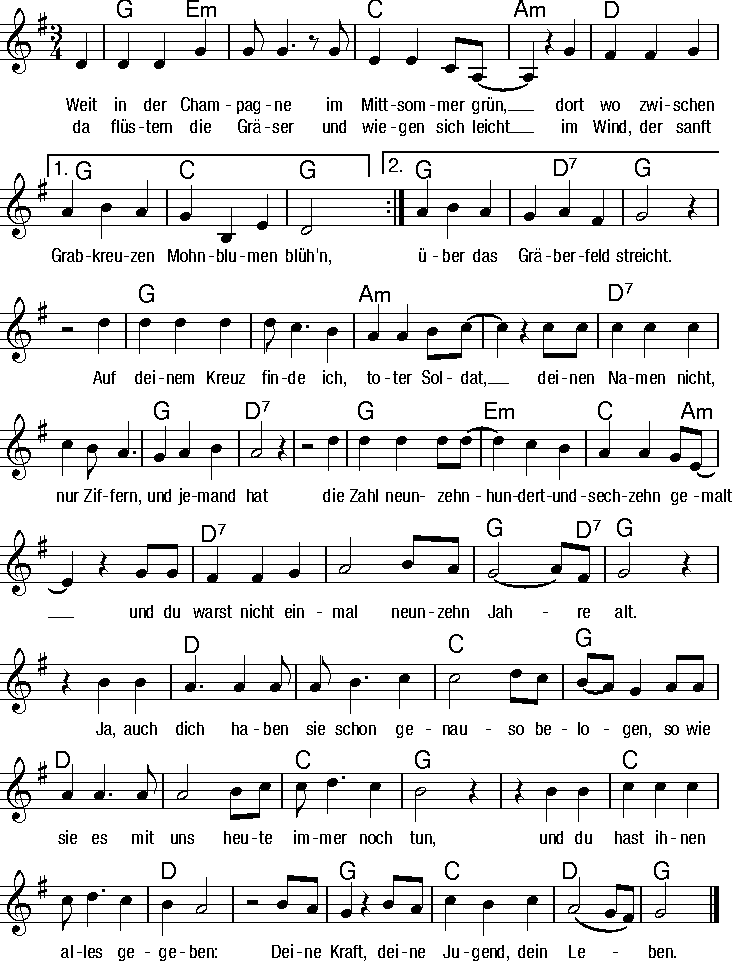
\includegraphics[width=1\textwidth]{Noten/Lied036.pdf}	

%\centering\includegraphics[width=1\textwidth]{Noten/Lied036_1.pdf}	

\beginverse\memorize
Hast du, \[G]toter Sol\[Em]dat, mal ein \[C]Mädchen ge\[Am]liebt?
Sicher \[D]nicht, denn nur dort, wo es \[G]Frie\[C]den \[G]gibt,
können \[G]Zärtlichkeit \[Em]und Ver\[C]trauen ge\[Am]deih'n.
Warst \[D]Soldat, um zu sterben, nicht \[G]um jung \[D7]zu \[G]sein.
Viel\[G]leicht dachtest du dir: Ich \[Am]falle schon bald,
nehme \[D7]mir mein Vergnügen, wie es \[G]kommt, mit Ge\[D7]walt.
Dazu \[G]warst du ent\[Em]schlossen, hast \[C]dich aber \[Am]dann
vor \[D7]dir selber geschämt und es doch \[G]nie \[D7]ge\[G]tan.
\endverse

\beginchorus
Ja, auch \[D]dich haben sie schon \[C]genauso \[G]belogen,
so, wie \[D]sie es mit uns heute \[C]immer noch \[G]tun,
und du \[C]hast ihnen alles \[D]gegeben:
Deine \[G]Kraft, deine \[C]Jugend, dein \[D]Le\[G]ben.
\endchorus

\beginverse
Sol^dat, gingst du ^gläubig und ^gern in den ^Tod?
Oder ^hast du verzweifelt, ver^bittert, ^ver^roht
deinen ^wirklichen ^Feind nicht er^kannt bis zum ^Schluss?
Ich ^hoffe, es traf dich ein ^saube^rer ^Schuss.
Oder ^hat ein Geschoss dir die ^Glieder zerfetzt?
Hast du ^nach deiner Mutter ge^schrien bis zu^letzt?
Bist du ^auf deinen ^Beinstümpfen ^weiterge^rannt?
Und dein ^Grab, birgt es mehr als ein ^Bein, ei^ne ^Hand?
\endverse

\beginchorus
Ja, auch \[D]dich haben sie schon \[C]genauso \[G]belogen,
so wie \[D]sie es mit uns heute \[C]immer noch \[G]tun,
und du \[C]hast ihnen alles \[D]gegeben:
Deine \[G]Kraft, deine \[C]Jugend, dein \[D]Le\[G]ben.
\endchorus

\beginverse
Es ^blieb nur das ^Kreuz als ^einzige ^Spur
^von deinem Leben, doch ^hör' mei^nen ^Schwur
für den ^Frieden zu ^kämpfen und ^wachsam zu ^sein.
Fällt die ^Menschheit noch einmal auf Lü^gen ^he^rein,
dann ^kann es gescheh'n, dass bald ^niemand mehr lebt,
niemand, ^der die Milliarden von ^Toten be^gräbt.
Doch längst ^finden sich ^mehr und mehr ^Menschen be^reit,
diesen ^Krieg zu verhindern, es ^ist an ^der ^Zeit.
\endverse

\beginchorus
Ja, auch \[D]dich haben sie schon \[C]genauso \[G]belogen,
so wie \[D]sie es mit uns heute \[C]immer noch \[G]tun,
und du \[C]hast ihnen alles \[D]gegeben:
Deine \[G]Kraft, deine \[C]Jugend, dein \[D]Le\[G]ben.
\endchorus

\endsong

\beginscripture{}
Das Lied ist die deutsche Variante von ''The green fields of France'' von Eric Bogle und wurde in dieser Version zu einer Hymne der Friedensbewegung in den 1980er Jahren.
\endscripture
